\documentclass[a4paper,12pt]{article} % тип документа

% Поля страниц
\usepackage[left=2.5cm,right=2.5cm,
    top=2cm,bottom=2cm,bindingoffset=0cm]{geometry}
    
%Пакет дял таблиц   
\usepackage{multirow} 
    
%Отступ после заголовка    
\usepackage{indentfirst}


% Рисунки
\usepackage{floatrow,graphicx,calc}
\usepackage{wrapfig}

%%% Работа с картинками
\usepackage{graphicx}  % Для вставки рисунков
\graphicspath{{images/}{images2/}}  % папки с картинками
\setlength\fboxsep{3pt} % Отступ рамки \fbox{} от рисунка
\setlength\fboxrule{1pt} % Толщина линий рамки \fbox{}
\usepackage{wrapfig} % Обтекание рисунков и таблиц текстом

% Создаёем новый разделитель
\DeclareFloatSeparators{mysep}{\hspace{1cm}}

% Ссылки?
\usepackage{hyperref}
\usepackage[rgb]{xcolor}
\hypersetup{				% Гиперссылки
    colorlinks=true,       	% false: ссылки в рамках
	urlcolor=blue          % на URL
}


%  Русский язык
\usepackage[T2A]{fontenc}			% кодировка
\usepackage[utf8]{inputenc}			% кодировка исходного текста
\usepackage[english,russian]{babel}	% локализация и переносы

% Математика
\usepackage{amsmath,amsfonts,amssymb,amsthm,mathtools}

%%% Дополнительная работа с математикой
\usepackage{amsmath,amsfonts,amssymb,amsthm,mathtools} % AMS
\usepackage{icomma} % "Умная" запятая: $0,2$ $-$- число, $0, 2$ $-$- перечисление


% Что-то 
\usepackage{wasysym}


\begin{document}
\begin{center}
	\footnotesize{МОСКОВСКИЙ ФИЗИКО-ТЕХНИЧЕСКИЙ ИНСТИТУТ\\(НАЦИОНАЛЬНЫЙ 			ИССЛЕДОВАТЕЛЬСКИЙ УНИВЕРСИТЕТ)}\\
	\footnotesize{ФИЗТЕХ-ШКОЛА РАДИОТЕХНИКИ И КОМПЬЮТЕРНЫХ ТЕХНОЛОГИЙ\\}
	\hfill \break
	\hfill \break
	\hfill \break
	\hfill \break
	\hfill \break
	\hfill \break
\end{center}

\begin{center}   
    \hfill \break
	\hfill \break
	\hfill \break
	\hfill \break
	\hfill \break
	\hfill \break
	\hfill \break
	\hfill \break
	\hfill \break
	\hfill \break
	\hfill \break
	\large{Лабораторная работа № 4.7.2\\\large{\textbf{Эффект Поккельса}}}\\
	\hfill \break
        \hfill \break
	\hfill \break
	\hfill \break
	\hfill \break
	\hfill \break
	\hfill \break
	\hfill \break
	\hfill \break
	\hfill \break
	\hfill \break
	\begin{flushright}
		Климова Екатерина\\
		Группа Б01-108
	\end{flushright}
	\hfill \break
\end{center}
\hfill \break
\hfill \break
\begin{center}
	Долгопрудный, 2023 г.
\end{center}
\thispagestyle{empty}

\newpage
\hfill \break
\textbf{Цель работы:} исследовать интерференцию рассеянного света, прошедшего кристалл; наблюдать изменение характера поляризации света при наложении на кристалл электрического поля.  
\hfill \break
\hfill \break
\textbf{В работе используются:} гелий-неоновый лазер; поляризатор; кристалл ниобата лития; матовая пластинка; экран; источник высоковольтного переменного и постоянного напряжения; фотодиод; осциллограф; линейка.

\section{Аннотация}
\hfill \break В работе предлагается: 1) измерив радиусы интерференционных колец, определить разность показателей преломления $n_{o} - n_{e}$; 2) подав на кристалл постоянное напряжение, получить свет, поляризованный по кругу; 3) определить полуволновое напряжение по фигурам Лиссажу на экране осциллографа.

\section{Теоретические сведения}
\subsection{Типы поляризации, основные понятия}
\hfill \break Плоские электромагнитные волны являются поперечными, то есть проекции осциллирующих электрического и магнитного полей на направление распространения такой волны равны нулю. Это непосредственно следует из теоремы Гаусса и теоремы о циркуляции магнитного поля. Пусть плоская электромагнитная волна распространяется в вакууме вдоль оси $z$. Тогда по теореме Гаусса:

$$
\text{div} \text{ } {\textbf{E}} = \frac {\partial E_{x}} {\partial x} + \frac {\partial E_{y}} {\partial y} + \frac {\partial E_{z}} {\partial z} = 0,
$$

\hfill \break но поскольку в рассматриваемой волне все производные по $x$ и по $y$ равны нулю, то и $\partial E_{z} / \partial z = 0$, то есть для $E_{z}$ равны нулю все пространственные производные. С другой стороны, из уравнения циркуляции магнитного поля следует, что 

$$
(\text{rot } {\textbf{H}})_{z} = \frac {\partial H_{y}} {\partial x} + \frac {\partial H_{x}} {\partial y} = \frac {1}{c} \frac {\partial E_{z}} {\partial t},
$$

\hfill \break то есть и $\partial E_{z} / \partial t = 0$ по той же причине, и, таким образом, $E_{z}$ является константой. Но поскольку мы рассматриваем осциллирующее поле с нулевым средним значением, эта константа равна нулю. Аналогично из теоремы Гаусса для магнитного поля и закона электромагнитной индукции получим $H_{z} = 0$.

\hfill \break Теперь, выписав из уравнения циркуляции магнитного поля и уравнения электромагнитной индукции выражения для оставшихся $x$- и $y$-компонент роторов $\textbf{E}$ и $\textbf{H}$ и воспользовавшись условием $E_{z} = H_{z} = 0$, мы увидим, что уравнения Максвелла для электрического и магнитного полей разделились на две независимые системы уравнений, одна из которых связывает $E_{x}$ и $H_{y}$, а другая $-$ $E_{y}$ и $H_{x}$:

$$
\begin{cases}
(\text{rot} \text{ } \textbf{E})_{y} = \frac {\partial E_{x}} {\partial z} = - \frac{1}{c} \frac {\partial H_{y}} {\partial t},
\\
(\text{rot} \text{ } \textbf{H})_{x} = \frac {\partial H_{y}} {\partial z} = - \frac{1}{c} \frac {\partial E_{x}} {\partial t},
\end{cases}
$$

\hfill \break и

$$
\begin{cases}
(\text{rot} \text{ } \textbf{E})_{x} = \frac {\partial E_{y}} {\partial z} = - \frac{1}{c} \frac {\partial H_{x}} {\partial t},
\\
(\text{rot} \text{ } \textbf{H})_{y} = \frac {\partial H_{x}} {\partial z} = - \frac{1}{c} \frac {\partial E_{y}} {\partial t}.
\end{cases}
$$

\hfill \break Решениями этих систем являются две независимые плоские волны вида $E_{x} \mp H_{y} = f_{x}(ct \pm z)$ и $E_{y} = \pm H_{x} = f_{y}(ct \pm z)$, где $f_{x}$ и $f_{y}$ $-$ произвольные функции. Важным частным случаем являются монохроматические волны:

\begin{equation}\label{ linkname }
E_{x} = H_{y} = A_{x} \cos{ (\omega t - kz + \varphi_{x} ) }
\end{equation}

\hfill \break или

\begin{equation}\label{ linkname }
E_{y} = - H_{x} = A_{y} \cos { (\omega t - kz + \varphi_{y})}.
\end{equation}

\hfill \break В любой точке пространства концы векторов в каждой из этих волн движутся по отрезкам прямых линий в плоскости $(E_{x}, \text{ } E_{y})$, поэтому они называются \textbf{линейно поляризованными (или плоскополяризованными)}. По историческим причинам плоскость, параллельно которой направлены вектора $\textbf{H}$, обычно называется плоскостью поляризации, а плоскость, параллельно которой направлены вектора $\textbf{E}$ $-$ плоскостью колебаний.

\hfill \break Если обе описанные выше монохроматические волны (1) и (2) распространяются одновременно, то концы векторов движутся по эллипсам в плоскости $(E_{x}, \text{ } E_{y})$. Это наиболее общий тип поляризации $-$ \textbf{эллиптическая поляризация}, все другие типы поляризации могут рассматриваться как его частный случай. Если полуоси эллипса равны, то такую поляризацию называют \textbf{круговой}. Различают правую и левую эллиптические поляризации. Свет называют правополяризованным, если для наблюдателя, смотрящего \textit{навстречу} лучу, вектор $\textbf{E}$ вращается по часовой стрелке. 

\subsection{Двойное лучепреломление}
\hfill \break \textbf{Двойное лучепреломление} в анизотропных кристаллах $-$ результат зависимости в этих кристаллах коэффициента преломления (и соответственно угла преломления, а также угла полного внутреннего отражения) от поляризации световой волны. 

\hfill \break В некоторых кристаллах потенциальные ямы, в которых находятся электроны вблизи узлов решетки, не являются сферически-симметричными. При этом систему координат всегда можно выбрать так, что для малых отклонений от положения равновесия потенциальная энергия электрона будет иметь вид

$$
U = a_{x} x^2 + a_{y} y^2 + a_{z} z^2.
$$

\hfill \break Если все три коэффициента различны, то кристалл называется двуосным, если два коэффициента равны $-$ одноосным, если равны все три коэффициента, то яма является сферически-симметричной, а вещество соответственно оптически изотропным. Наибольшее практическое значение имеют одноосные кристаллы. Положим $a_{y} = a_{z} = a_{\perp}$, $a_{x} = a_{||}$. Ось $x$ при этом называется \textbf{оптической осью кристалла}.

\hfill \break Поскольку отклонения от положения равновесия под действием внешнего поля у электронов вдоль разных осей координат обратно пропорциональны соответствующим коэффициентам в выражении для потенциальной энергии, то вектор удельного дипольного момента $P$ и, как следствие, вектор электрической индукции $D$ окажутся в общем случае неколлинеарны вектору напряженности электрического поля $E$:

\begin{equation}\label{ linkname }
P = \alpha_{\perp} E_{\perp} + \alpha_{||}E_{||}, \text{ } D = \varepsilon_{\perp}E_{\perp} + \varepsilon_{||}E_{||}.
\end{equation}

\hfill \break Здесь $\alpha_{\perp}$, $\alpha_{||}$ $-$ поляризуемости, $\varepsilon_{||} = 1 + 4\pi \alpha_{||}$, $\varepsilon_{\perp} = 1 + 4\pi \alpha_{\perp}$ $-$ диэлектрические проницаемости кристалла вдоль и поперек его оптической оси соответственно.

\hfill \break Распространение электромагнитных волн описывается уравнениями Максвелла, которые в отсутствие электрических зарядов и токов имеют вид

$$
\text{rot} \text{ } H = \frac{1}{c} \frac {\partial D} {\partial t}, \text{ } \text{rot} \text{ } E = - \frac{1}{c} \frac {\partial H} {\partial t}.
$$

\hfill \break Определим, при каких условиях в одноосных кристаллах могут распространяться плоские монохроматические электромагнитные волны. Такие волны в общем случае можно записать в виде:

$$
E = E_{0}e^{i(\omega t - kr)}, \text{ } H = H_{0} e^{i(\omega t - kr)}, \text{ } D = D_{0} e^{i(\omega t - kr)},
$$

\begin{wrapfigure}{l}{0.25\textwidth}
\begin{center}
    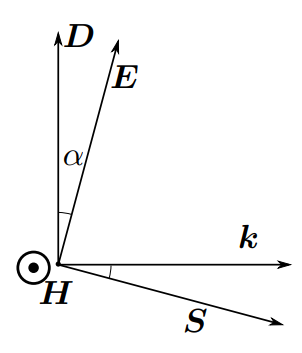
\includegraphics[width=1\textwidth]{4.7.2_1.png}
    \textbf{Рис. 1.} Расположение векторов $D$, $E$, $k$, $S$ в анизотропной среде
\end{center}
\end{wrapfigure}

\hfill \break откуда следует $\text{rot} \text{ } H = -ik \times H$, $\frac {\partial D} {\partial t} = i \omega D$ и аналогичные выражения для других векторов. Подставив эти выражения в выписанные выше уравнения Максвелла, получим, что $D$, $H$ и $E$ должны быть связаны соотношениями

\begin{equation}\label{ linkname }
D = - \frac{c}{\omega} k \times H, \text{ } H = \frac{c}{\omega}k \times E,
\end{equation}

\hfill \break отсюда видно, что векторы $D$, $H$, $k$ взаимно перпендикулярны, то есть плоские волны поперечны в отношении $D$ и $H$, но в общем случае не поперечны в отношении $E$. Кроме того, вектор $E$ должен лежать в одной плоскости с векторами $D$ и $k$, так как все они перпендикулярны $H$. 

\hfill \break Взаимное расположение векторов $D$, $E$, $k$, а также вектора плотности потока энергии (Пойнтинга) $S = \frac{4\pi}{c} E \times H$ показано на рис. 1.

\hfill \break Несложный геометрический анализ показывает, что одновременное выполнение условий (4) и материального уравнения (3) $D = \varepsilon_{\perp}E_{\perp} + \varepsilon_{||}E_{||}$ возможно только в двух случаях (рис. 2).

\begin{itemize}
    \item Если вектор $D$ перпендикулярен плоскости, в которой лежат оптическая ось кристалла и волновой вектор (эта плоскость называется \textbf{главным сечением}).
    \item Если вектор $D$ лежит в главном сечении.
\end{itemize}

\begin{center}
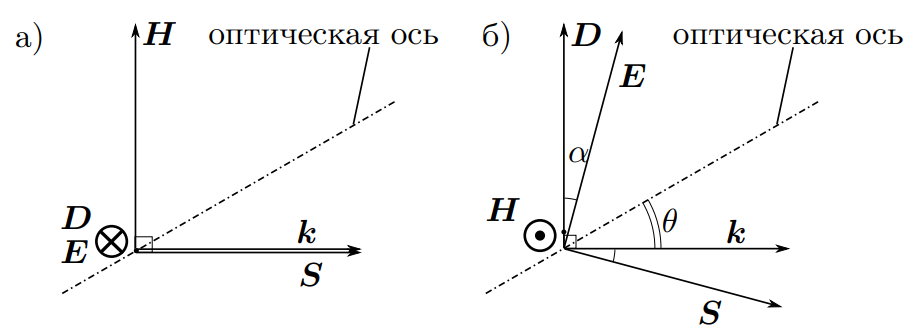
\includegraphics[width=0.65\textwidth]{4.7.2_2.png}\\
\textbf{Рис. 2.} Обыкновенная (а) и необыкновенная (б) волны и положение основных векторов в них; плоскость рисунка $-$ главное сечение \\
\end{center}

\hfill \break В первом случае плоская волна называется \textbf{обыкновенной}, а во втором $-$ \textbf{необыкновенной} волной. Во всех остальных случаях электромагнитное поле неизбежно имеет более сложный вид, чем простая плоская монохроматическая волна. Поскольку уравнения Максвелла линейны, в общем случае любое монохроматическое поле в кристалле можно представить в виде суперпозиции обыкновенной и необыкновенной волн.

\hfill \break Обыкновенная и необыкновенная волны распространяются в кристалле с разной скоростью. У обыкновенной волны $E_{||} = 0$, $E = E_{\perp}$, значит, векторы индукции и напряженности электрического поля коллинеарны: $D = \varepsilon_{\perp}E_{\perp}$, поэтому вид уравнений Максвелла для нее ничем не отличается от уравнений для плоских волн в изотропных средах. Следовательно, фазовая скорость $v = \omega/k$ этой волны не зависит от направления $k$ и равна

\begin{equation}\label{ linkname }
v_{o} = \frac{c} {\sqrt{\varepsilon_{\perp}}} = \frac{c}{n_{o}},
\end{equation}

\hfill \break где $n_{o} = \sqrt{\varepsilon_{\perp}}$ $-$ коэффициент преломления для обыкновенной волны.

\hfill \break У необыкновенной волны векторы индукции и напряженности электрического поля в общем случае неколлинеарны, а фазовая скорость такой волны зависит от угла $\theta$ между оптической осью и волновым вектором. Квадрат коэффициента преломления есть уже не отношение модулей $D/E$, а отношение модуля $D$ и проекции $E_{D} = E \cos{\alpha}$ вектора $E$ на направление вектора $D$:

\begin{equation}\label{ linkname }
D = \varepsilon E_{D}, \text{ } v_{e} = \frac{c}{\sqrt{\varepsilon}} = \frac {c} {n(\theta)}, \text{ где } \varepsilon = \frac {1} {\frac {\sin{\theta}^2} {\varepsilon_{||}} + \frac {\cos{\theta}^2}{\varepsilon_{\perp}} },
\end{equation}

\hfill \break $n(\theta) = \sqrt{\varepsilon}$ $-$ коэффициент преломления необыкновенной волны, зависящий от угла $\theta$ между оптической осью и волновым вектором. Кроме того, у необыкновенной волны вектор Пойнтинга и групповая скорость не коллинеарны в общем случае волновому вектору, то есть направление переноса энергии и направление смещения поверхностей равных фаз не совпадает.

\hfill \break Плоская монохроматическая волна, попадающая из изотропной среды в анизотропный одноосный кристалл, распадается в общем случае на две взаимно ортогонально поляризованные плоские волны, распространяющиеся в общем случае в разных направлениях и с разными скоростями.

\subsection{Эффект Поккельса}
\hfill \break \textbf{Эффектом Поккельса} называется изменение показателя преломления света в кристалле под действием электрического поля, причём это изменение пропорционально напряжённости электрического поля. Как следствие эффекта Поккельса в кристалле появляется двойное лучепреломление или меняется его величина, если кристалл был двулучепреломляющим в отсутствие поля.

\begin{center}
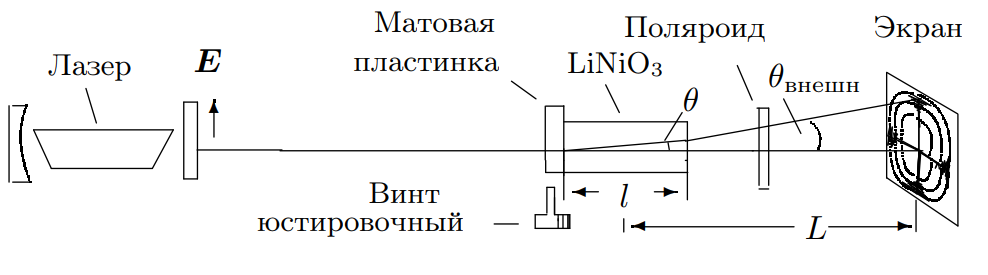
\includegraphics[width=0.75\textwidth]{4.7.2_3.png}\\
\textbf{Рис. 3.} Схема для наблюдения интерференционной картины \\
\end{center}
	
\hfill \break Рассмотрим сначала кристалл LiNbO$_3$ в отсутствие внешнего электрического поля. Кристалл ниобата лития является одноосным кристаллом, то есть кристаллом, оптические свойства которого обладают симметрией вращения относительно некоторого одного направления, называемого оптической осью $Z$ кристалла. 

\hfill \break Для световой волны, вектор электрического поля $\vec{E}$ которой перпендикулярен оси $Z$, показатель преломления равен $n_o$, а для волны, вектор $\vec{E}$ которой располагается вдоль оси $Z$, он равен $n_e$, причём $n_e < n_o$, т. е. LiNbO$_3$ $-$ «отрицательный кристалл». В общем случае, когда луч света распространяется под углом $\theta$ к оптической оси $Z$ (рис. 3), существуют два собственных значения показателя преломления $n_1$ и $n_2$: если световой вектор $\vec{E}$ перпендикулярен плоскости $(\vec{k},\vec{Z})$, где $\vec{k}$ $-$ волновой вектор луча, то волна называется обыкновенной («$o$» $-$ ординарная), а показатель преломления $n_1$ равен $n_o$ и не зависит от угла $\theta$; когда световой вектор $\vec{E}$ лежит в плоскости $(\vec{k}, \text{ } \vec{Z})$ $-$ это необыкновенная («$e$» $-$ экстраординарная) волна, при этом показатель преломления $n_2$ зависит от угла $\theta$ и определяется уравнением
	
\begin{equation*}
	\frac{1}{n_2^2} = \frac{\cos^2\theta}{n_o^2} + \frac{\sin^2\theta}{n_e^2}.
\end{equation*}
	
\hfill \break Если перед кристаллом, помещённым между скрещенными поляроидами (рис. 3), расположить линзу или матовую пластинку, после которых лучи будут рассеиваться под различными углами, то на экране, расположенном за поляроидом, мы увидим тёмные концентрические окружности (коноскопическую картину) $-$ результат интерференции обыкновенной и необыкновенной волн, точнее, проекцию их электрических полей на разрешённое направление выходного поляроида.

\hfill \break Разность фаз между обыкновенной и необыкновенной волнами, приобретаемая при прохождении через кристалл длиной $l$, равна
	
 \begin{equation}
	\Delta \varphi = \frac{2\pi}{\lambda} l (n_1 - n_2).
\end{equation}

\hfill \break Для обыкновенного луча $n_1 = n_o$. Считая, что $n_e$ и $n_o$ отличаются незначительно, для малых углов $(\sin\theta \approx \theta, \text{ } \cos\theta \approx 1 - \theta^2/2)$ получаем $n_2$ $=$ $n_o - (n_o - n_e)\theta^2$. Таким образом,
	
\begin{equation}
	\delta = \frac{2\pi}{\lambda}l(n_o - n_e)\theta^2.
\end{equation}

\hfill \break Если $L$ $-$ расстояние от центра кристалла до экрана, то, учитывая закон преломления (закон Снеллиуса) на границе кристалла, при малых углах $\theta_{\text{внешн}} = n_o \theta$ (рис. 3) получаем выражение для \textbf{радиуса кольца}:
	
\begin{equation}
	r_m^2 = \frac{\lambda}{l}\frac{(n_o L)^2}{(n_o - n_e)}m.
\end{equation}

\hfill \break При перпендикулярных ориентациях лазера и анализатора имеем:
	
\begin{equation}
	I_{\text{вых}} = I_0\sin^2\left(\frac{\pi}{2}\frac{U}{U_{\lambda / 2}}\right), 
\end{equation}

\hfill \break где $U_{\lambda / 2} = \frac{\lambda}{4A} \frac{d}{l}$ $-$ \textbf{полуволновое напряжение}.

\hfill \break При параллельных:
	
\begin{equation}
	I_{\text{вых}} = I_0\cos^2\left(\frac{\pi}{2}\frac{U}{U_{\lambda / 2}}\right).
\end{equation}

\section{Экспериментальная установка}
\hfill \break Оптическая часть установки представлена на рис. 3. Свет гелий-неонового лазера, поляризованный в вертикальной плоскости, проходя сквозь матовую пластинку, рассеивается и падает на двоякопреломляющий кристалл под различными углами. Кристалл ниобата лития с размерами $3 \times 3 \times 26$ мм вырезан вдоль оптической оси $z$. На экране, расположенном за скрещенным поляроидом, видна интерференционная картина.

\begin{center}
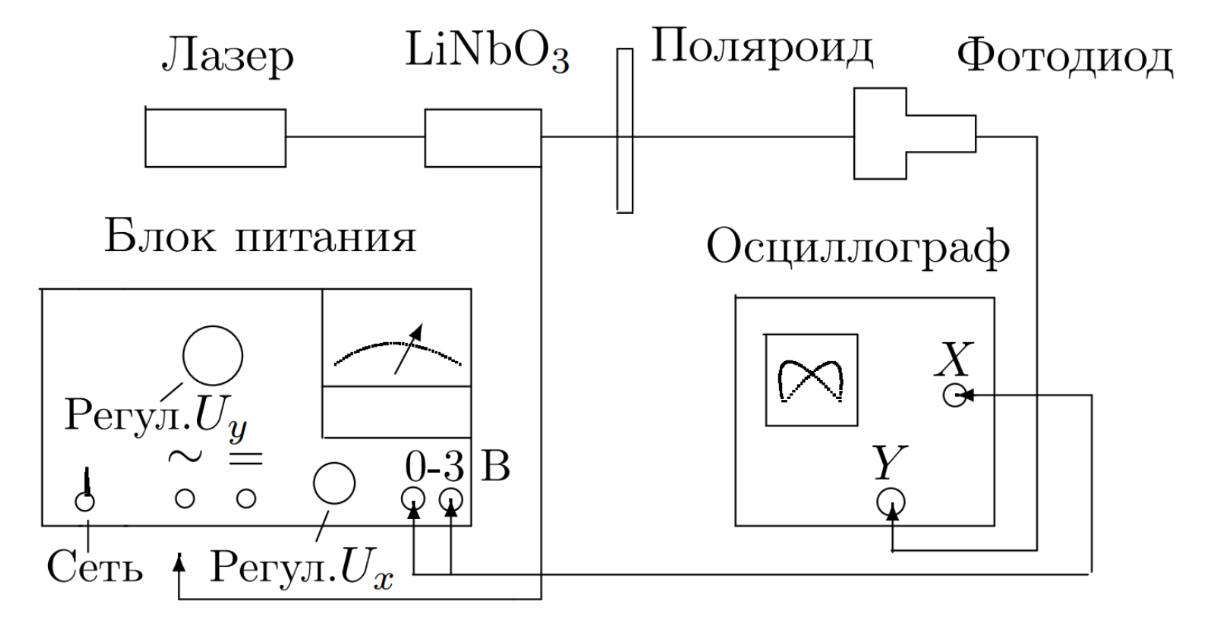
\includegraphics[width=0.65\textwidth]{4.7.2_4.png}\\
\textbf{Рис. 4.} Схема для изучения двойного лучепреломления в электрическом поле \\
\end{center}

\hfill \break Для $\lambda = 0.63$ мкм (длина волны гелий-неонового лазера) в ниобате лития $n_{o} = 2.29$.

\hfill \break Убрав рассеивающую пластинку и подавая на кристалл постоянное напряжение, можно величиной напряжения влиять на поляризацию луча, вышедшего из кристалла.

\hfill \break Заменив экран фотодиодом (рис. 4) и подав на кристалл переменное напряжение, можно исследовать поляризацию луча с помощью осциллографа.

\section{Ход работы}
\hfill \break Соберем оптическую схему согласно рис. 3. Включим лазер и установим анализатор (без кристалла в схеме) так, чтобы лазерное излучение через него не проходило (скрещенные поляризации). Чтобы убедиться, что лазерный луч поляризован вертикально, определим разрешенное направление анализатора: посмотрим сквозь поляроид на дневной свет от окна, отраженный от светлой поверхности; вращая поляроид, найдем минимум освещенности и заметим отсчет угла на лимбе. Вблизи угла Брюстера в отраженном свете преобладает компонента светового вектора, параллельная плоскости стола, следовательно, минимум отраженного света соответствует вертикальному разрешененному направлению поляроида. 

\hfill \break Поставим кристалл и установим перед ним вплотную к кювете матовую пластинку. Получим на экране интерференционную картину. Отклоняя кристалл с помощью юстировочного винта и поворачивая рейтер с кюветой вокруг вертикальной оси, добьемся совмещения центра коноскопической картины с положением луча на экране в отсутствие матовой пластинки. Повернем анализатор на 90 градусов и убедимся, что коноскопическая картина изменилась на негативную. Вернем анализатор в прежнее положение (горизонтальное разрешенное направление).

\hfill \break Перейдем к измерениям. Зафиксируем расстояние от середины кристалла до экрана $L = (96 \pm 1)$ см, измерим радиусы темных колец $r(m)$ и занесем их в таблицу:

\begin{center}
\begin{tabular}{|c|c|c|}\hline
$ m $ & $ r_{m} $, см & $ r_{m}^2 $, $ \text{мм}^2 $ \\\hline
1 & 2.5 & 6.25 \\\hline
2 & 4.2 & 17.64 \\\hline
3 & 5.3 & 28.09 \\\hline
4 & 6.3 & 39.69 \\\hline
5 & 7.1 & 50.41 \\\hline
6 & 7.8 & 60.84 \\\hline
7 & 8.4 & 70.56 \\\hline
8 & 9.0 & 81.00 \\\hline
9 & 9.5 & 90.25 \\\hline
\end{tabular} \\
\hfill \break \textbf {Таблица 1.} Радиусы темных колец \\
\end{center}

\hfill \break Построим график зависимости $r^2 = f(m)$:

\begin{center}
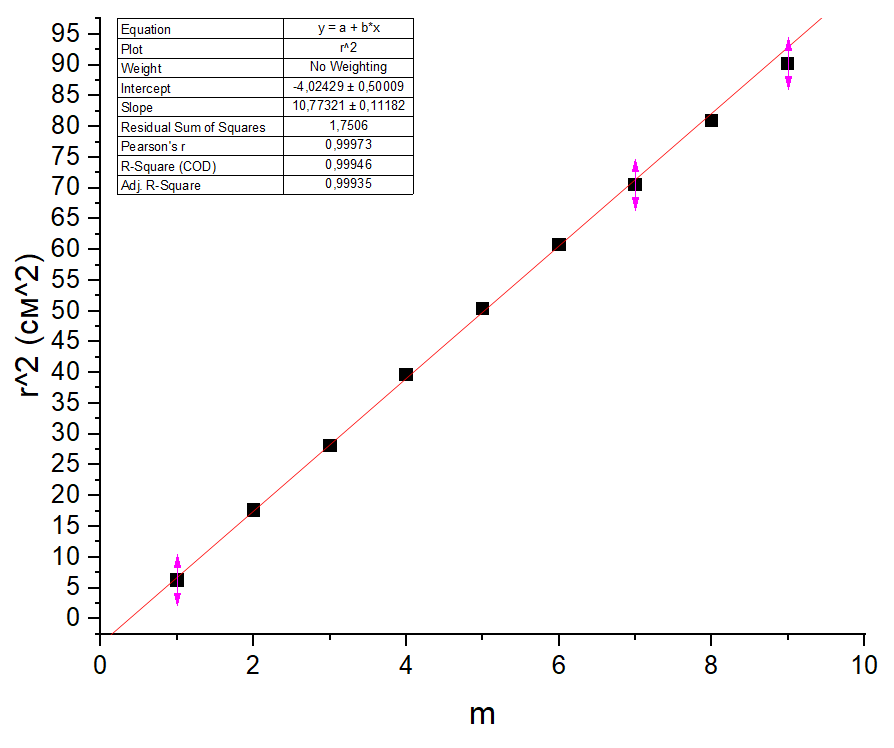
\includegraphics[width=0.70\textwidth]{4.7.2_5.png}\\
\textbf{Рис. 5.} График зависимости квадрата радиуса кольца от его порядка \\
\end{center}

\hfill \break Видим, что коэффициент наклона данного графика $k = 10.8 \pm 0.2$. Воспользуемся формулой (9): 

$$
n_{o} - n_{e} = \frac {\lambda n_{o}^2 L^2 m} {l r_{m}^2} = \frac {\lambda}{l} \cdot \frac {(n_{o}L)^2} {k},
$$

\hfill \break где $L = 0.96$ м, $\lambda = (6.3 \cdot 10^{-7})$ м $-$ длина волны гелий-неонового лазера, $n_{o} = 2.29$, $l = 0.026$ м $-$ длина кристалла. Тогда получаем \textit{двулучепреломление ниобата лития} $(n_{o} - n_{e}) = (0.106 \pm 0.004)$. Табличное значение $(n_{o} - n_{e})_{\text{табл}} \approx 0.09$, что достаточно близко к экспериментальному с учетом погрешности.

\hfill \break Уберем матовую пластинку и подключим разъем блока питания на постоянное напряжение, установим регулятор напряжения на минимальное напряжение и включим блок питания в сеть. С увеличением напряжения на кристалле яркость пятна на экране увеличивается и достигает максимума при $U = U_{\lambda/2}$. При $U = 2U_{\lambda/2} = U_{\lambda}$ яркость снова будет минимальной и так далее. Определим \textit{полуволновое напряжение ниобата лития}: $U_{\lambda/2} = 480$ В. 

\hfill \break Подадим на кристалл напряжение $U = \frac{1}{2} U_{\lambda/2} = U_{\lambda/4} = 240$ В (четвертьволновое напряжение). Поляризация на выходе кристалла должна быть круговой. Убедимся в этом, вращая анализатор и наблюдая за яркостью пятна на экране. Она не меняется, поэтому поляризация и правда круговая. 

\hfill \break Установим вместо экрана фотодиод (рис. 4) и подключим его к $y$-входу осциллографа. Убрав напряжение до нуля, переключим разъем на переменное напряжение. С трехвольтового выхода блока питания подадим сигнал на вход $x$ осциллографа. Отклонение луча осциллографа по оси $x$, таким образом, будет пропорционально напряжению $U$ на кристалле, а по оси $y$ $-$ интенсивности прошедшего через анализатор сигнала. 

\hfill \break Постепенно повышая напряжение на кристалле, будем наблюдать на экране осциллографа фигуры Лиссажу, соответствующие зависимости $I_{\text{вых}}(U)$ для скрещенных поляризаций лазера и анализатора. Определим по ним полуволновое напряжение как $\Delta U$, соответствующее переходу от максимума к минимуму сигнала на осциллограмме. Получили $U_{\lambda/2} = 480$ В, что идеально совпадает с полученным ранее значением.

\hfill \break \begin{center}
\begin{tabular}{ccc}
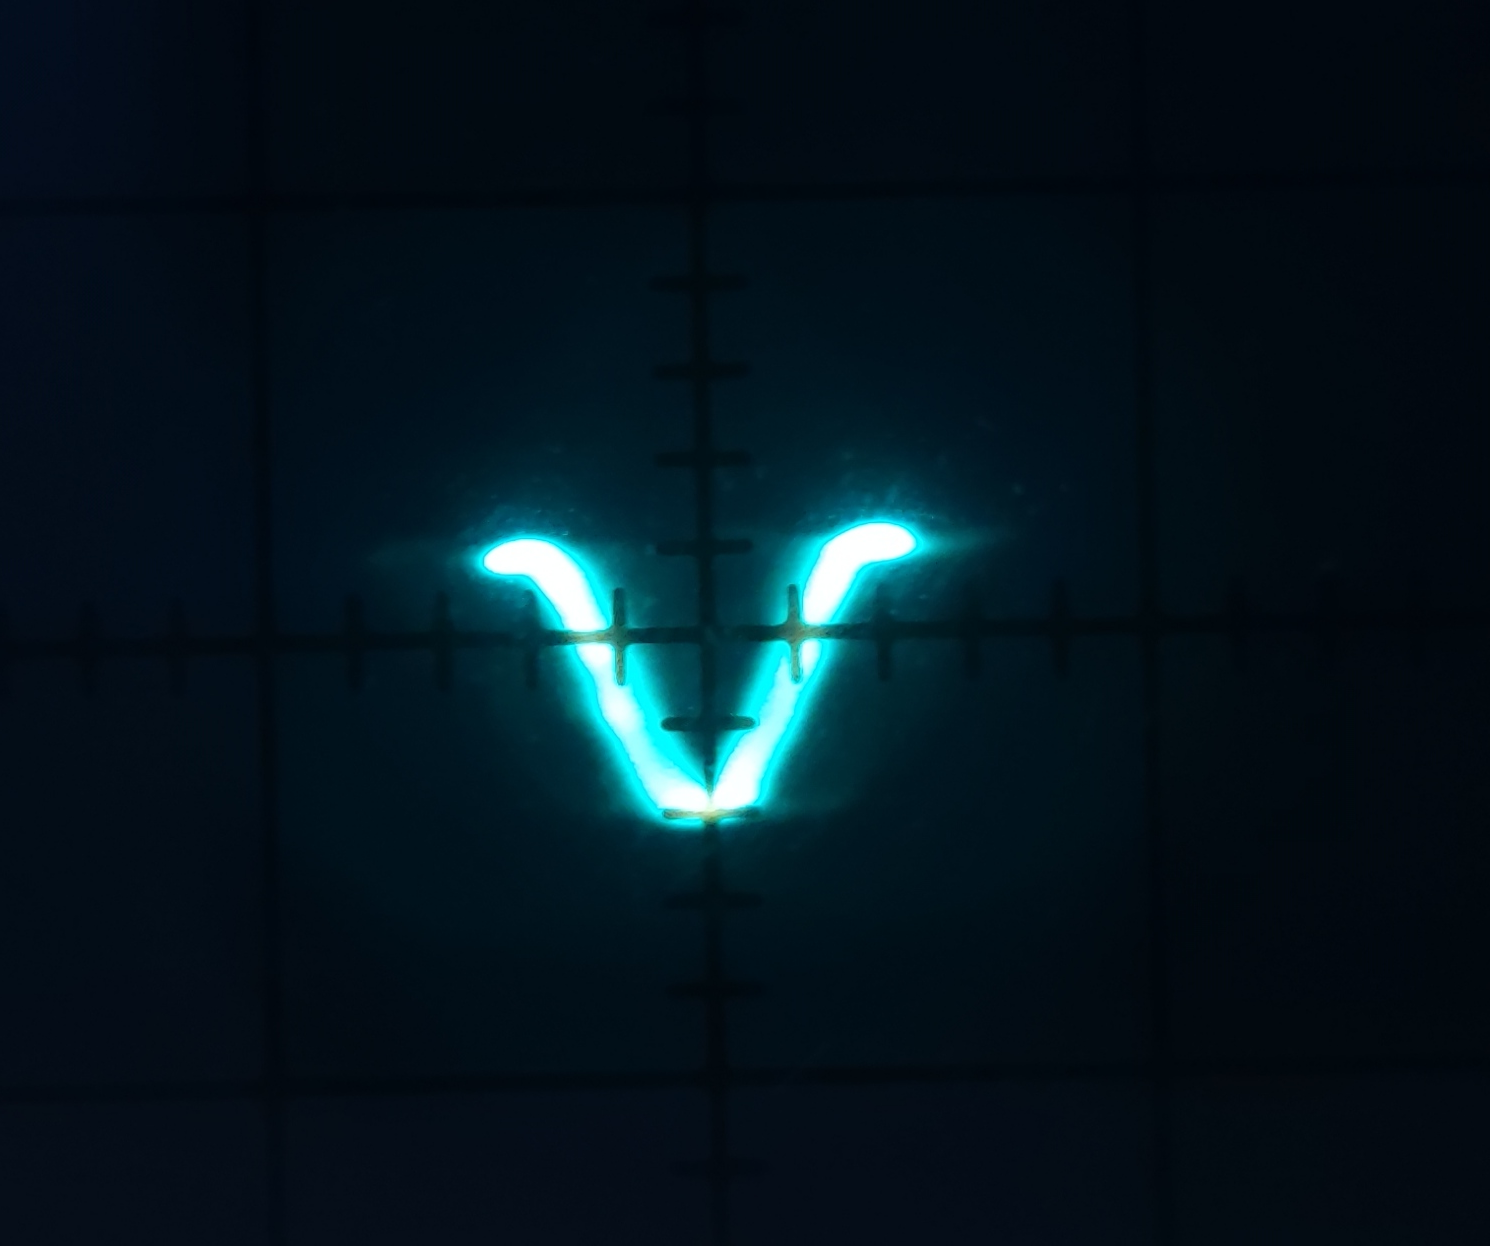
\includegraphics[width=0.3\textwidth]{4.7.2_6.png}&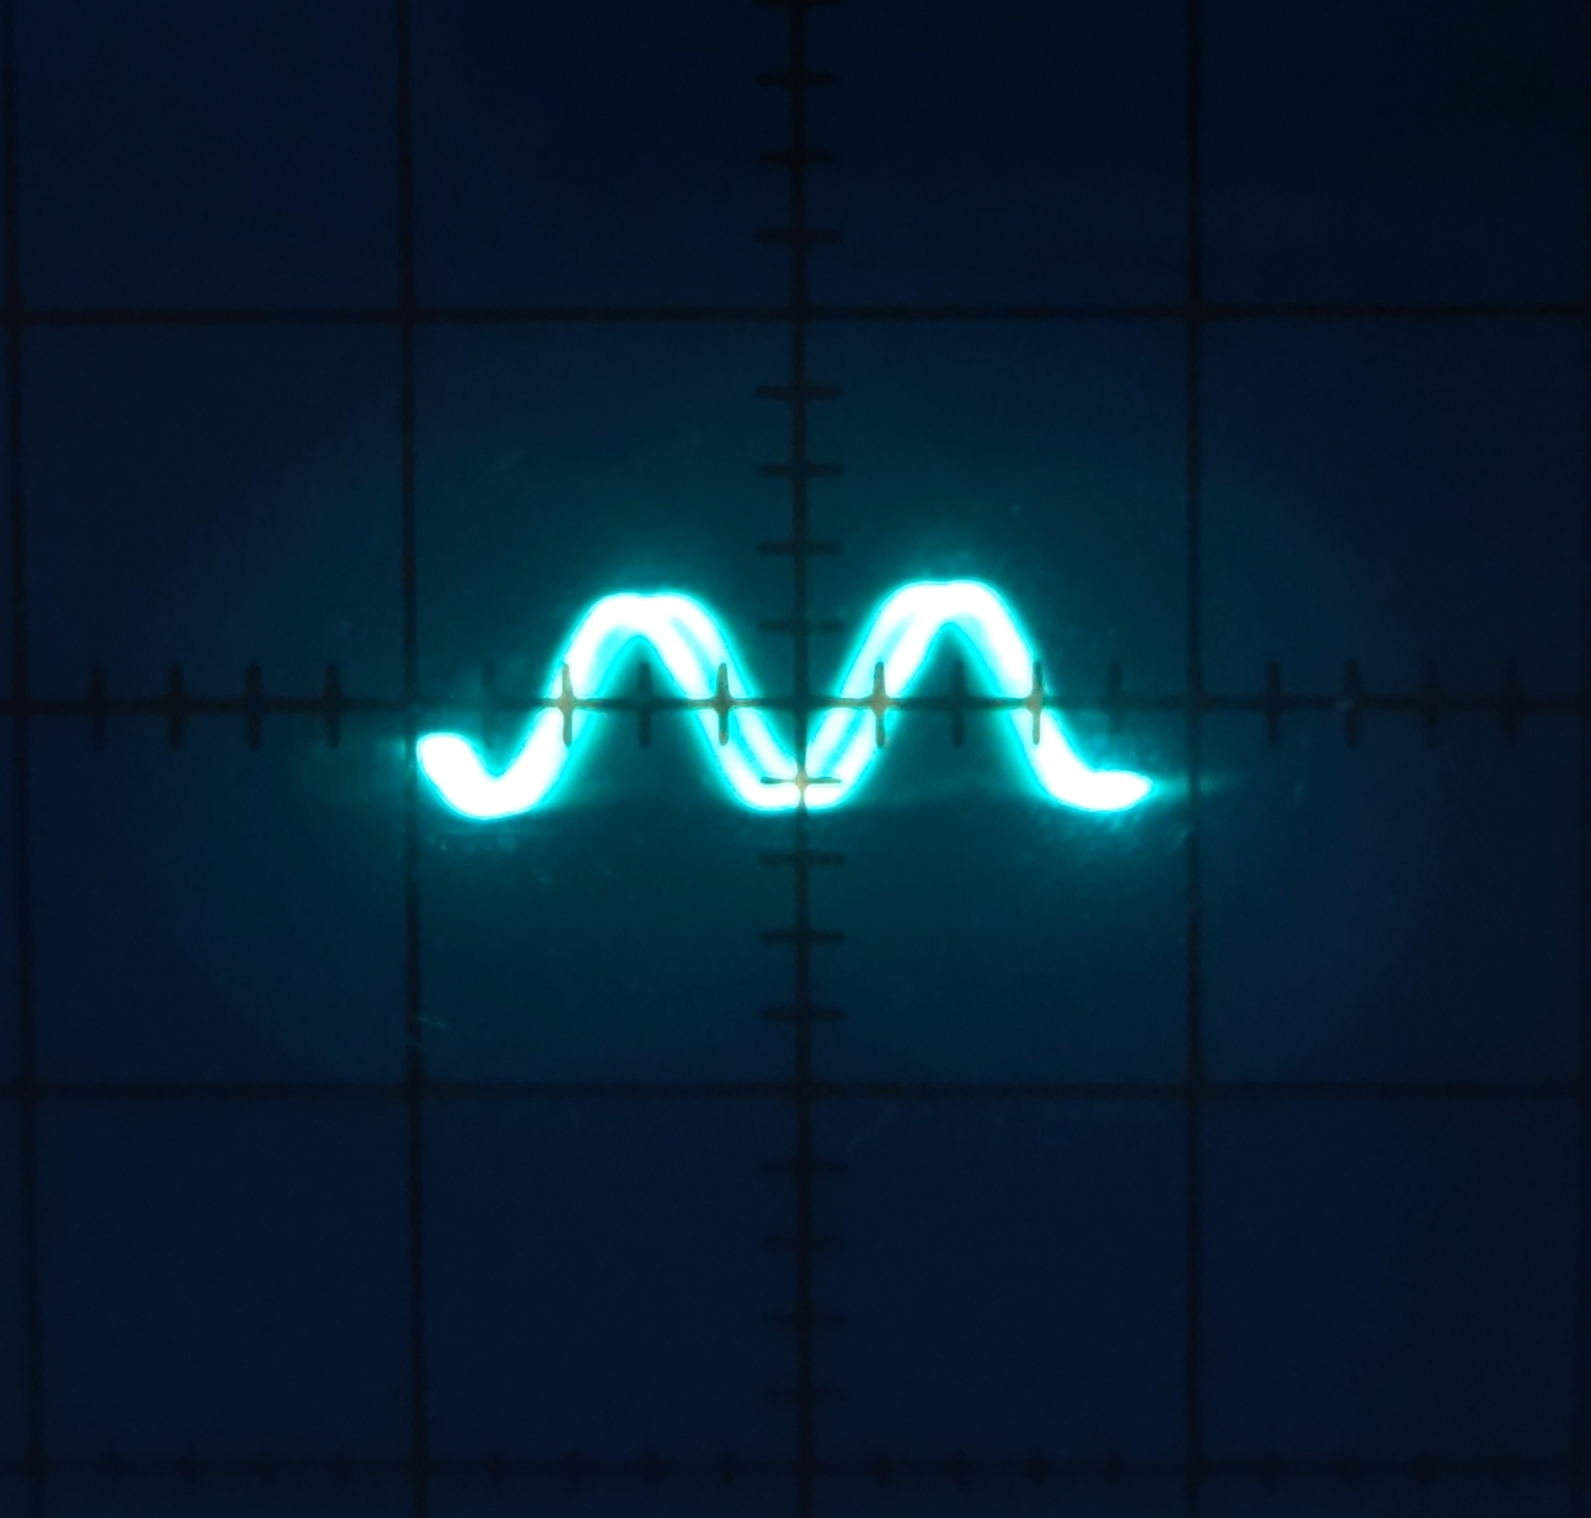
\includegraphics[width=0.3\textwidth]{4.7.2_7.png}&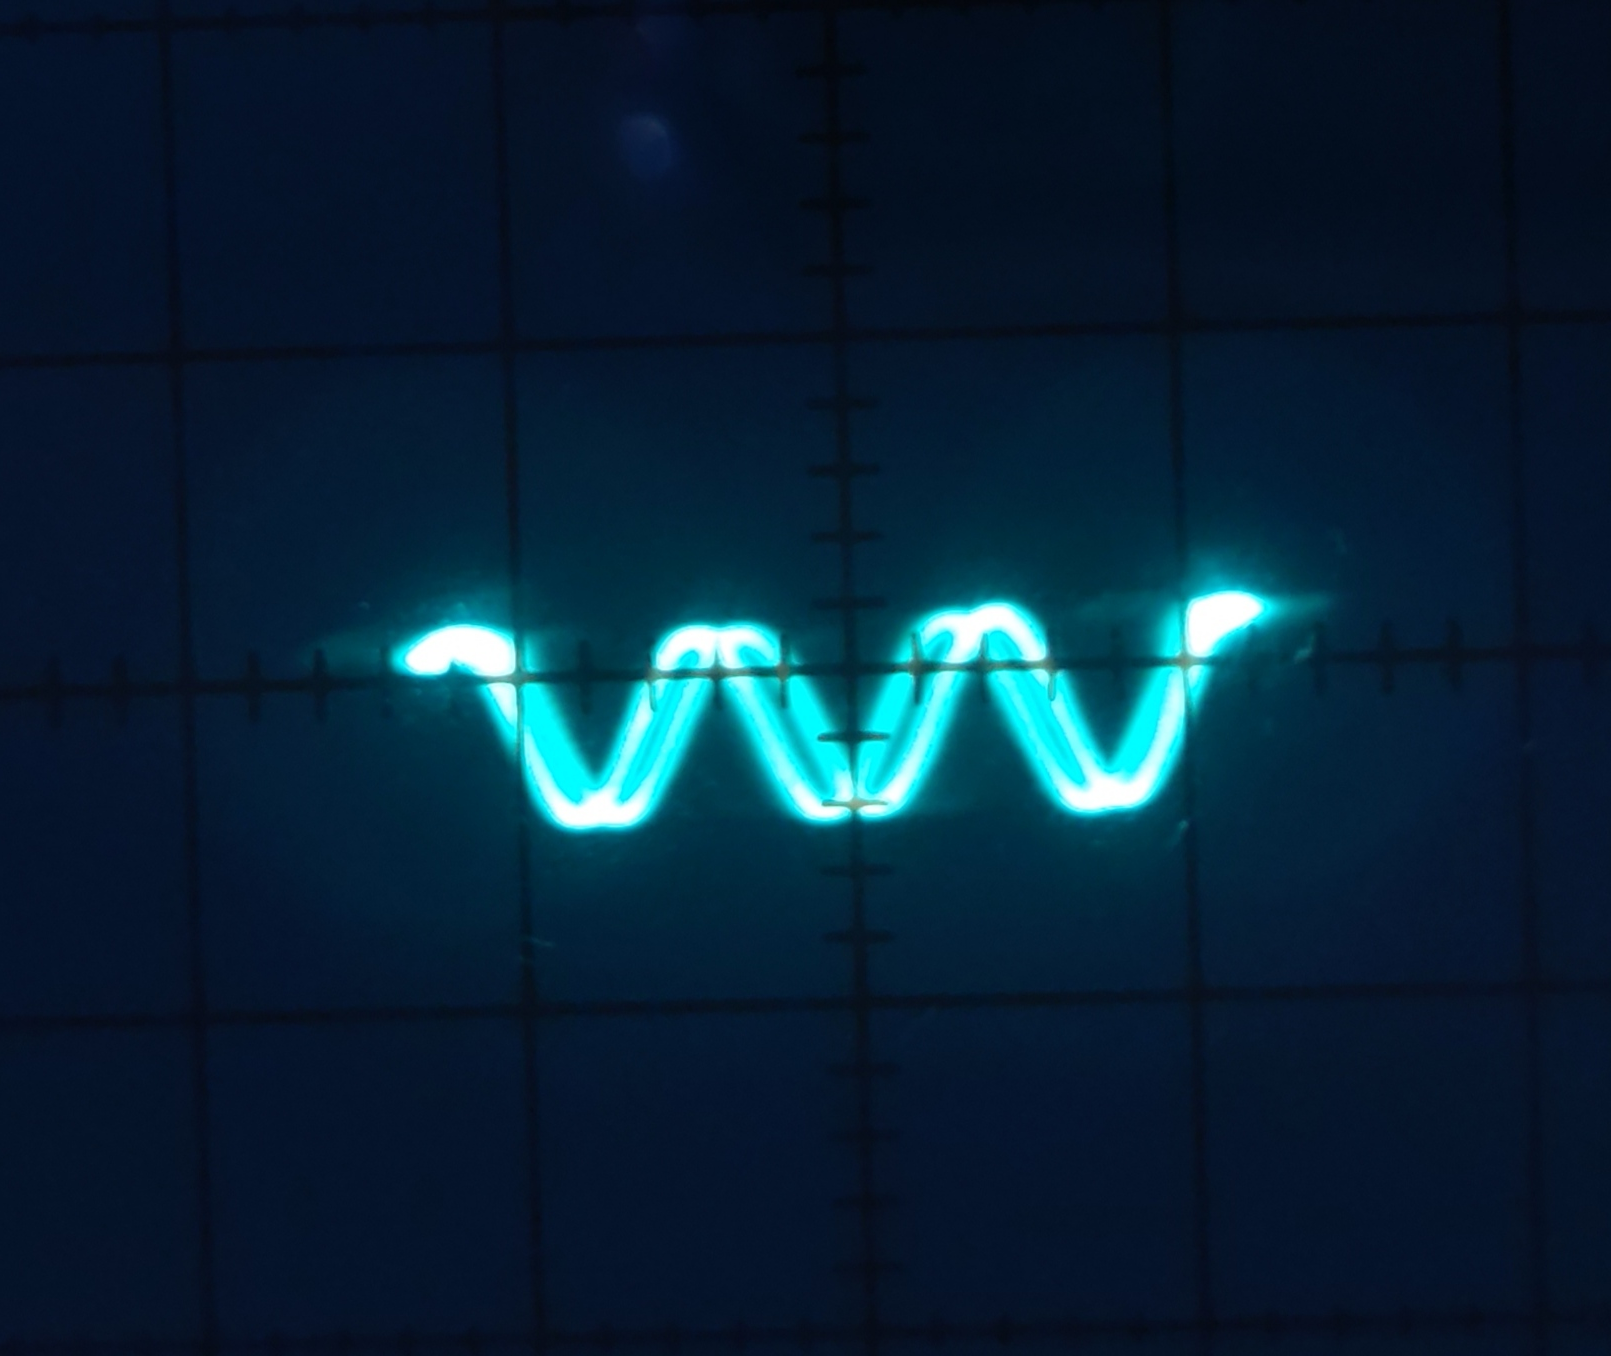
\includegraphics[width=0.3\textwidth]{4.7.2_8.png}\\
а) & б) & в)\\
\end{tabular}
\hfill \break \textbf {Рис. 6} Фигуры Лиссажу для напряжений $U_{\lambda/2}$ (а), $U_{\lambda}$ (б) и $U_{3\lambda/2}$ (в) \\
\end{center}

\section{Вывод}

\hfill \break В работе была изучена интерференция рассеянного света, прошедшего кристалл ниобата лития: получена зависимость квадрата радиуса темных колец интерференционной картины от номера минимума, с хорошей точностью являющаяся линейной, что согласуется с теорией при малых углах отклонения луча от оптической оси кристалла и близких значениях показателей преломления для обыкновенной и необыкновенной волн. Действительно, двулучепреломление кристалла $n_o - n_e$ составляет $(0.106 \pm 0.004)$, это значение неплохо сходится с табличным.
	
\hfill \break Также был рассмотрен эффект Поккельса: несколькими способами определено полуволновое напряжение, оно совпадает в пределах погрешности и равно $U_{\lambda/2} \approx 480$ В. Получены фигуры Лиссажу, отражающие зависимость интенсивности выходного сигнала от подаваемой амплитуды напряжения $I(U)$ при скрещенных и параллельных поляризациях. Картинки для поляризаций отличаются по фазе на $\pi/2$.

\end{document}
